\begin{figure}[htbp]
\centering
\begin{tikzpicture}[x=1cm,y=1cm]
\node[anchor=south west,inner sep=0] at (0,0) {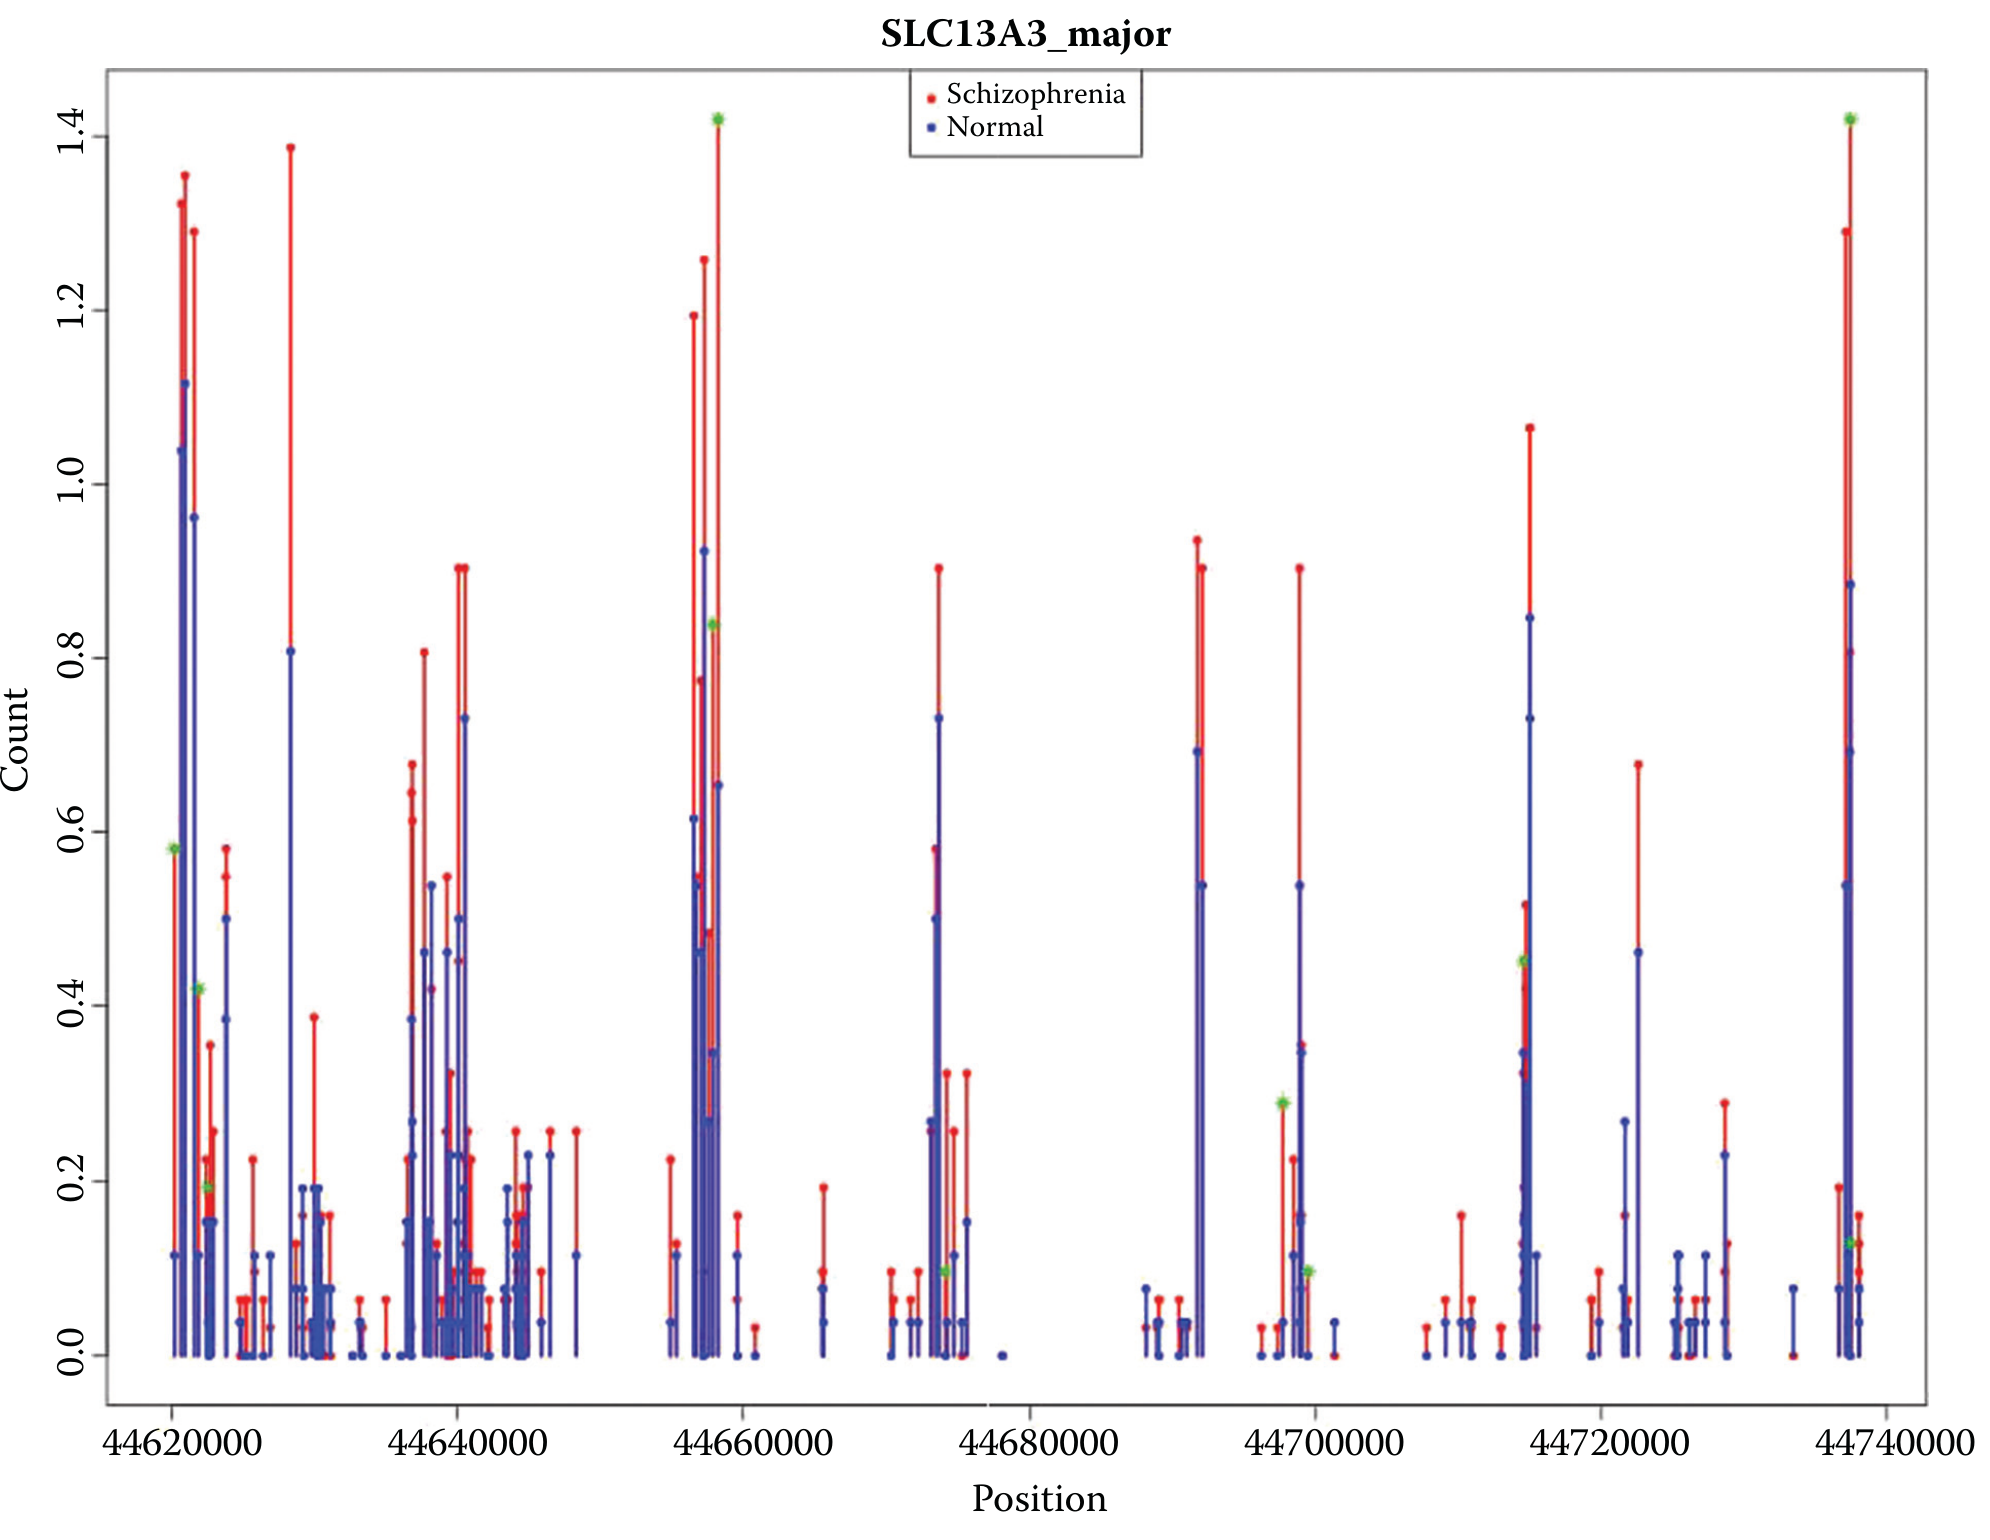
\includegraphics[width=12.0cm]{figures/ch04a_fig14_data.png}};
\fill[white] (5.6838,8.5975) rectangle (6.8152,8.8284);
\node[inner sep=0pt,fill=white,rotate=0,font=\fontsize{6}{8}\selectfont] at (6.2495,8.7130) {精神分裂症};
\fill[white] (5.6838,8.3947) rectangle (6.3195,8.6256);
\node[inner sep=0pt,fill=white,rotate=0,font=\fontsize{6}{8}\selectfont] at (6.0016,8.5101) {正常};
\fill[white] (-0.1054,4.4797) rectangle (0.3708,5.1653);
\node[inner sep=0pt,fill=white,rotate=90,font=\fontsize{8}{8}\selectfont] at (0.0652,4.8225) {计数};
\fill[white] (5.8321,0.0904) rectangle (6.7057,0.3816);
\node[inner sep=0pt,fill=white,rotate=0,font=\fontsize{8}{8}\selectfont] at (6.2689,0.2360) {位置};
\fill[white] (5.2844,8.9268) rectangle (7.0899,9.2180);
\node[inner sep=0pt,fill=white,rotate=0,font=\fontsize{8}{8}\selectfont] at (6.1872,9.0724) {SLC13A3：主要等位基因};
\end{tikzpicture}
\origfig{14}{基因 SLC13A3 主要等位基因的差异表达。}
\label{fig:ch04a-14}
\end{figure}
